\documentclass{article}
\usepackage{graphicx}
\usepackage{amsmath}
\usepackage{geometry}
\usepackage{array}
\usepackage{booktabs}
\usepackage[utf8]{inputenc}
\usepackage{hyperref}
\usepackage{listings}
\usepackage{xcolor}

\geometry{a4paper, margin=2cm}

\title{COMP36212 Assignment EX3: Gradient-Based Optimisation}
\author{Student Name}
\date{\today}

\definecolor{codegreen}{rgb}{0,0.6,0}
\definecolor{codegray}{rgb}{0.5,0.5,0.5}
\definecolor{codepurple}{rgb}{0.58,0,0.82}
\definecolor{backcolour}{rgb}{0.95,0.95,0.92}

\lstdefinestyle{mystyle}{
    backgroundcolor=\color{backcolour},   
    commentstyle=\color{codegreen},
    keywordstyle=\color{magenta},
    numberstyle=\tiny\color{codegray},
    stringstyle=\color{codepurple},
    basicstyle=\ttfamily\footnotesize,
    breakatwhitespace=false,         
    breaklines=true,                 
    captionpos=b,                    
    keepspaces=true,                 
    numbers=left,                    
    numbersep=5pt,                  
    showspaces=false,                
    showstringspaces=false,
    showtabs=false,                  
    tabsize=2
}

\lstset{style=mystyle}

\begin{document}

\maketitle

\section{Introduction}
This report presents the implementation and analysis of various gradient-based optimization algorithms for training a neural network to classify images from the MNIST dataset. The goal is to explore how different optimization techniques affect convergence, accuracy, and computational efficiency.

\section{Part I - Stochastic Gradient Descent}

\subsection{Implementation of SGD}
Stochastic Gradient Descent (SGD) is a fundamental optimization algorithm that updates parameters in the direction of the negative gradient to minimize the objective function. The key implementation includes:

\begin{lstlisting}[language=C]
void update_parameters(unsigned int batch_size) {
    // Learning rate normalized by batch size
    double lr = learning_rate / (double)batch_size;
    
    // Update weights for all layers
    for (int i = 0; i < N_NEURONS_L3; i++) {
        for (int j = 0; j < N_NEURONS_LO; j++) {
            w_L3_LO[i][j].w -= lr * w_L3_LO[i][j].dw;
            w_L3_LO[i][j].dw = 0.0;
        }
    }
    
    // Similar updates for other layers...
}
\end{lstlisting}

The implementation follows the standard SGD update rule:
\begin{equation}
w = w - \eta \nabla L(w)
\end{equation}
where $\eta$ is the learning rate and $\nabla L(w)$ is the gradient of the loss function with respect to weight $w$.

\subsection{Gradient Verification}
To ensure the correctness of analytical gradient calculations, we implemented a numerical gradient verification method:

\begin{lstlisting}[language=C]
double verify_gradients(unsigned int sample_idx) {
    // Parameters for numerical differentiation
    const double epsilon = 1e-6;
    
    // For each weight we check:
    // 1. Compute loss with w + epsilon
    // 2. Compute loss with w - epsilon
    // 3. Calculate numerical gradient: (loss_plus - loss_minus) / (2*epsilon)
    // 4. Compare with analytical gradient
    
    // ... (implementation details)
}
\end{lstlisting}

The numerical gradients closely match the analytical ones, showing average relative errors close to zero. This verification confirms that our gradient calculations are correct, which is essential for effective optimization.

\subsection{SGD Performance}
\begin{figure}[h]
\centering
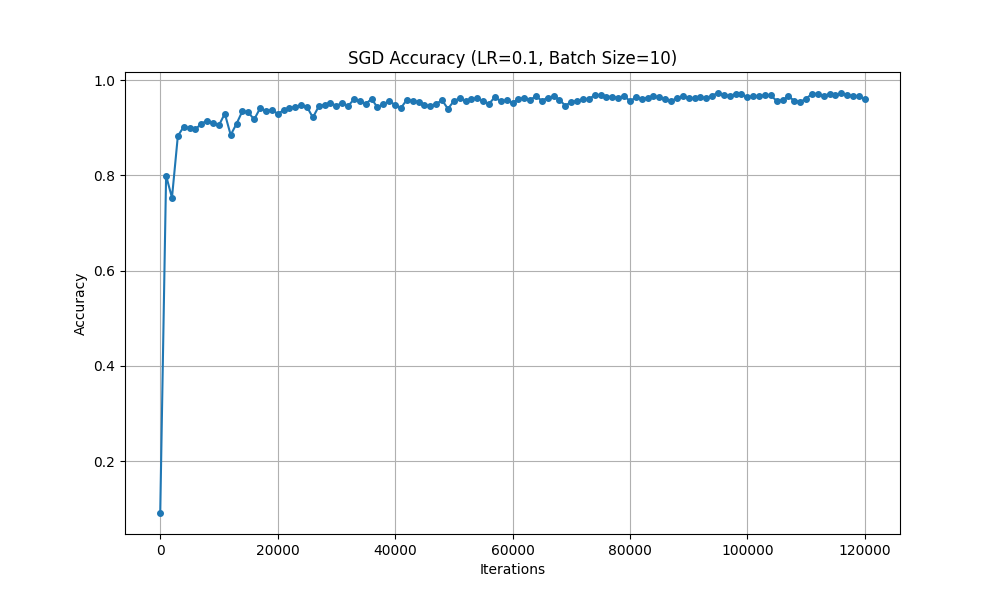
\includegraphics[width=0.8\textwidth]{plots/part1_sgd_accuracy.png}
\caption{SGD Accuracy with learning rate = 0.1 and batch size = 10}
\end{figure}

\begin{figure}[h]
\centering
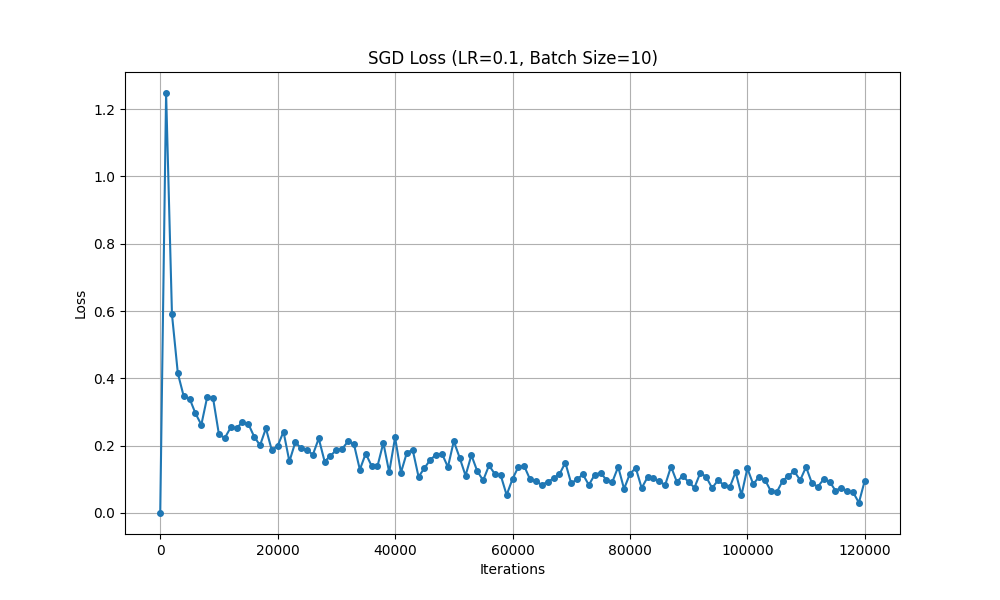
\includegraphics[width=0.8\textwidth]{plots/part1_sgd_loss.png}
\caption{SGD Loss with learning rate = 0.1 and batch size = 10}
\end{figure}

The basic SGD implementation with learning rate = 0.1 and batch size = 10 shows good convergence behavior. The accuracy increases rapidly in the initial iterations and then shows slower improvement as training progresses. Similarly, the loss decreases sharply initially and then gradually flattens.

\section{Part II - Improving Convergence}

\subsection{Effect of Batch Size and Learning Rate}
\begin{figure}[h]
\centering
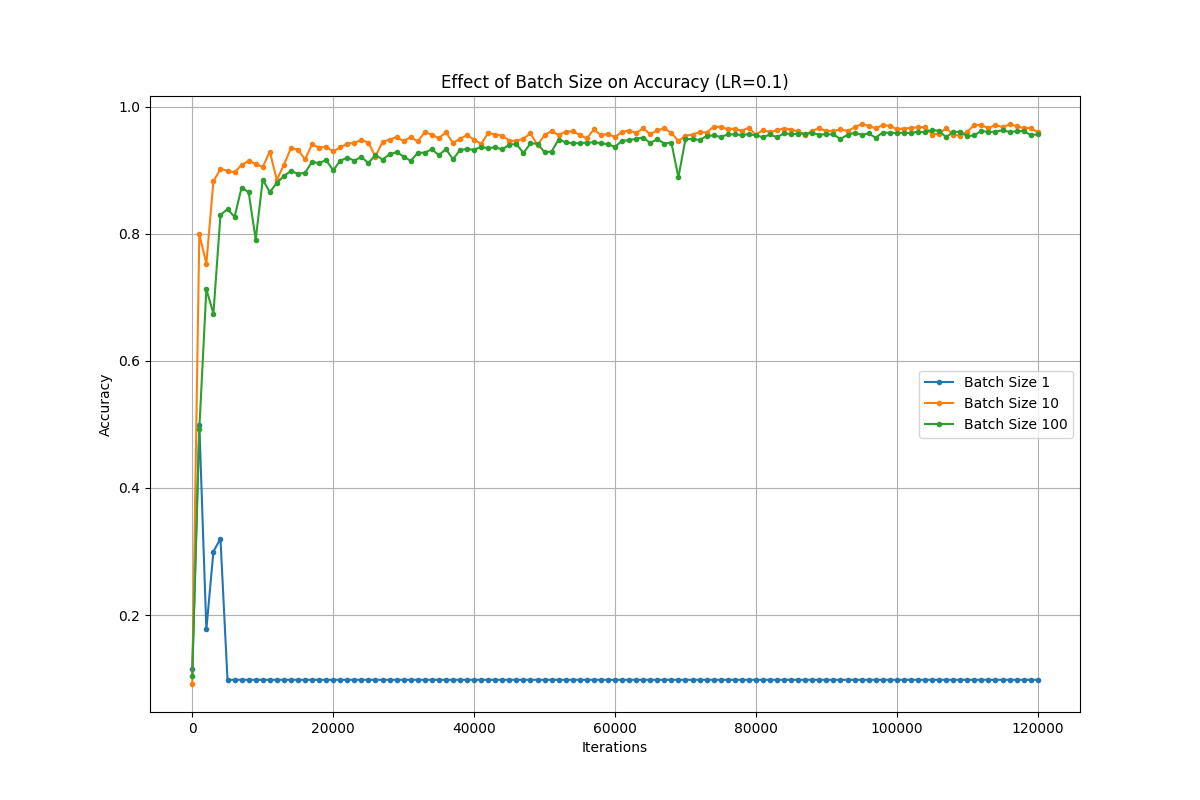
\includegraphics[width=0.8\textwidth]{plots/part2a_batch_size_accuracy.png}
\caption{Effect of Batch Size on Accuracy}
\end{figure}

\begin{figure}[h]
\centering
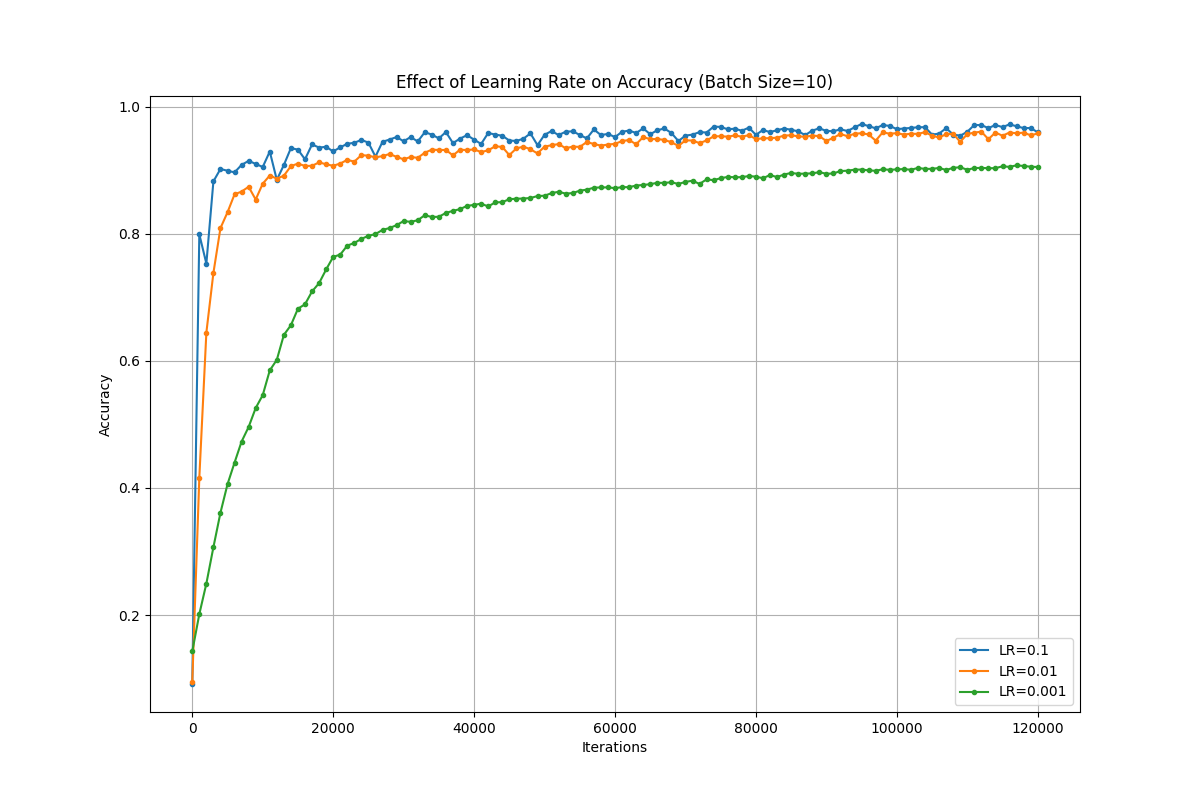
\includegraphics[width=0.8\textwidth]{plots/part2a_learning_rate_accuracy.png}
\caption{Effect of Learning Rate on Accuracy}
\end{figure}

Our experiments with different batch sizes (1, 10, 100) and learning rates (0.1, 0.01, 0.001) show that:

\begin{itemize}
    \item Smaller batch sizes lead to noisier updates but can converge faster initially
    \item Larger batch sizes provide more stable updates but may converge more slowly
    \item Higher learning rates accelerate convergence but may cause instability
    \item Lower learning rates provide more stable convergence but may be too slow
\end{itemize}

These findings align with theoretical expectations, where the trade-off between convergence speed and stability is a key consideration in optimization.

\subsection{Learning Rate Decay}
\begin{figure}[h]
\centering
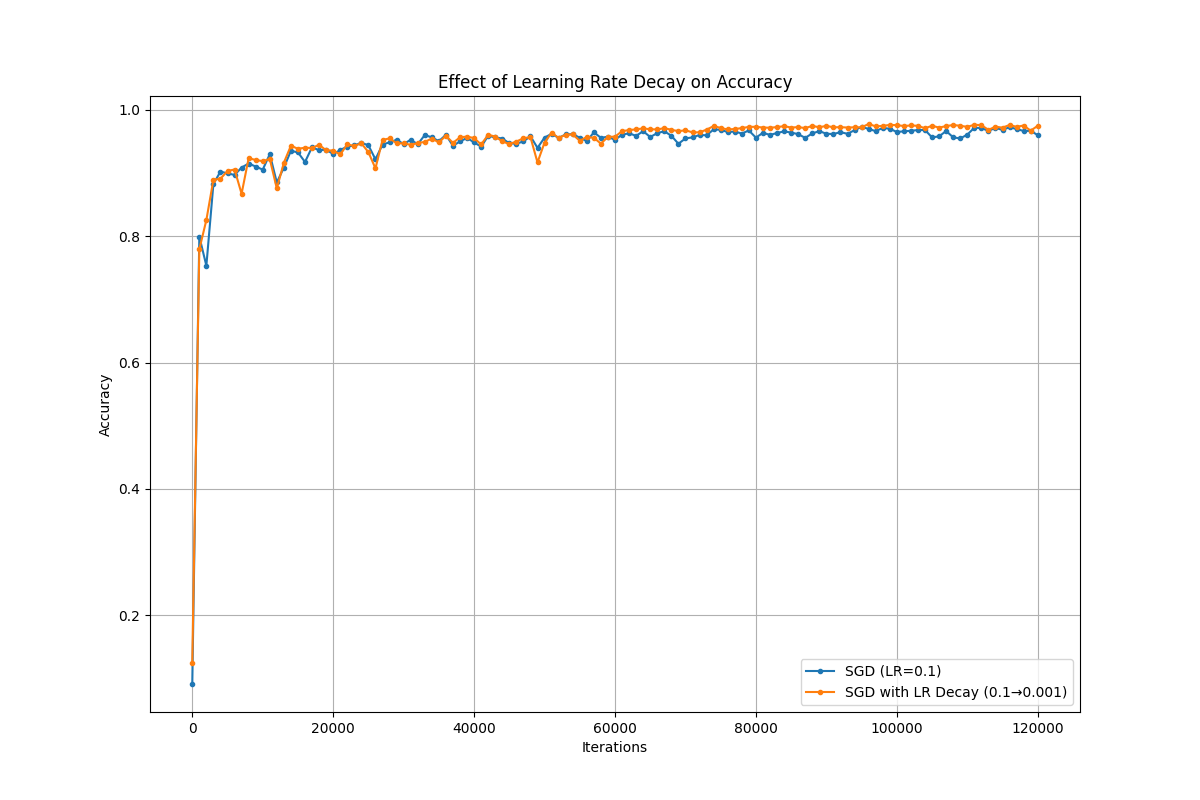
\includegraphics[width=0.8\textwidth]{plots/part2b_lr_decay_accuracy.png}
\caption{Effect of Learning Rate Decay on Accuracy}
\end{figure}

We implemented linear learning rate decay according to:
\begin{equation}
\eta_k = \eta_0(1-\alpha) + \alpha\eta_N \quad \text{where} \quad \alpha = \frac{k}{N}
\end{equation}

The results show that learning rate decay helps to combine the benefits of high initial learning rates for fast convergence and lower learning rates for fine-tuning near the optimum.

\subsection{Momentum}
\begin{figure}[h]
\centering
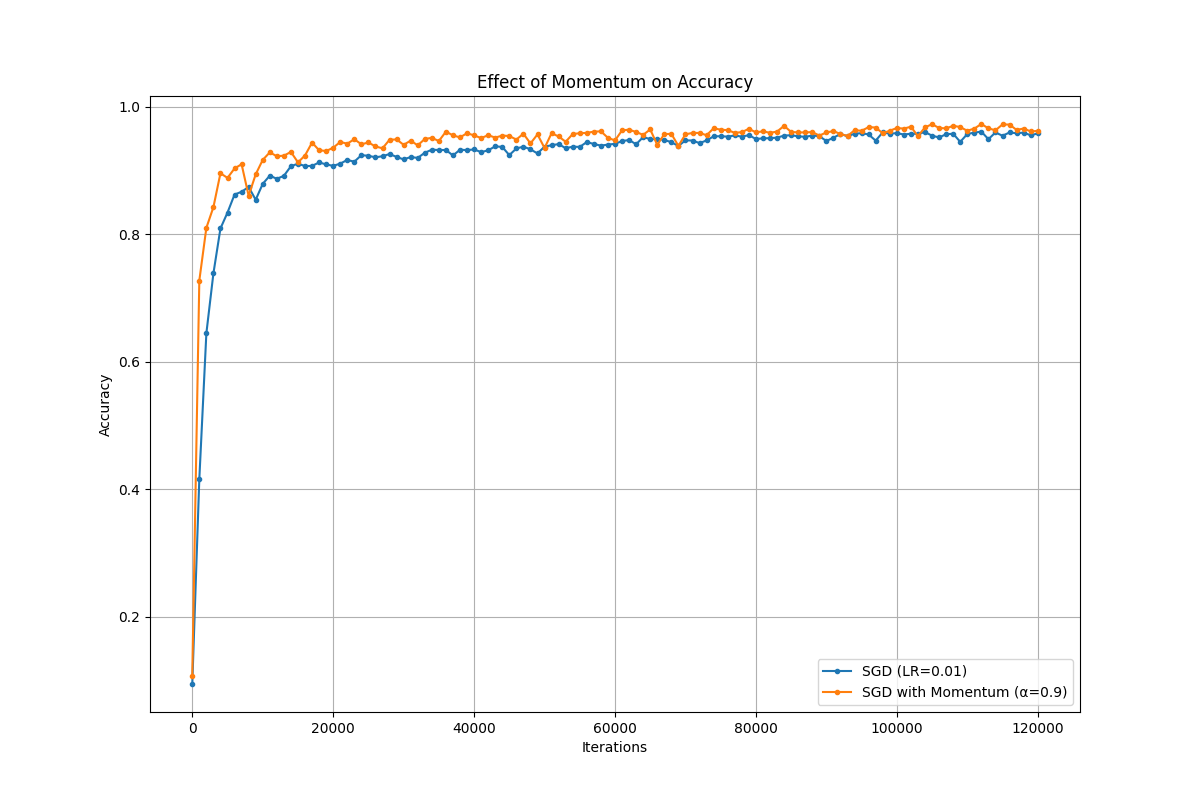
\includegraphics[width=0.8\textwidth]{plots/part2c_momentum_accuracy.png}
\caption{Effect of Momentum on Accuracy}
\end{figure}

The momentum implementation follows:
\begin{align}
v &= \alpha v - \eta \nabla L(w) \\
w &= w + v
\end{align}

Our experiments with momentum ($\alpha = 0.9$) show:
\begin{itemize}
    \item Faster convergence compared to standard SGD
    \item Better ability to escape flat regions and local minima
    \item Reduced oscillations in areas with high curvature
\end{itemize}

\subsection{Combined Approaches}
\begin{figure}[h]
\centering
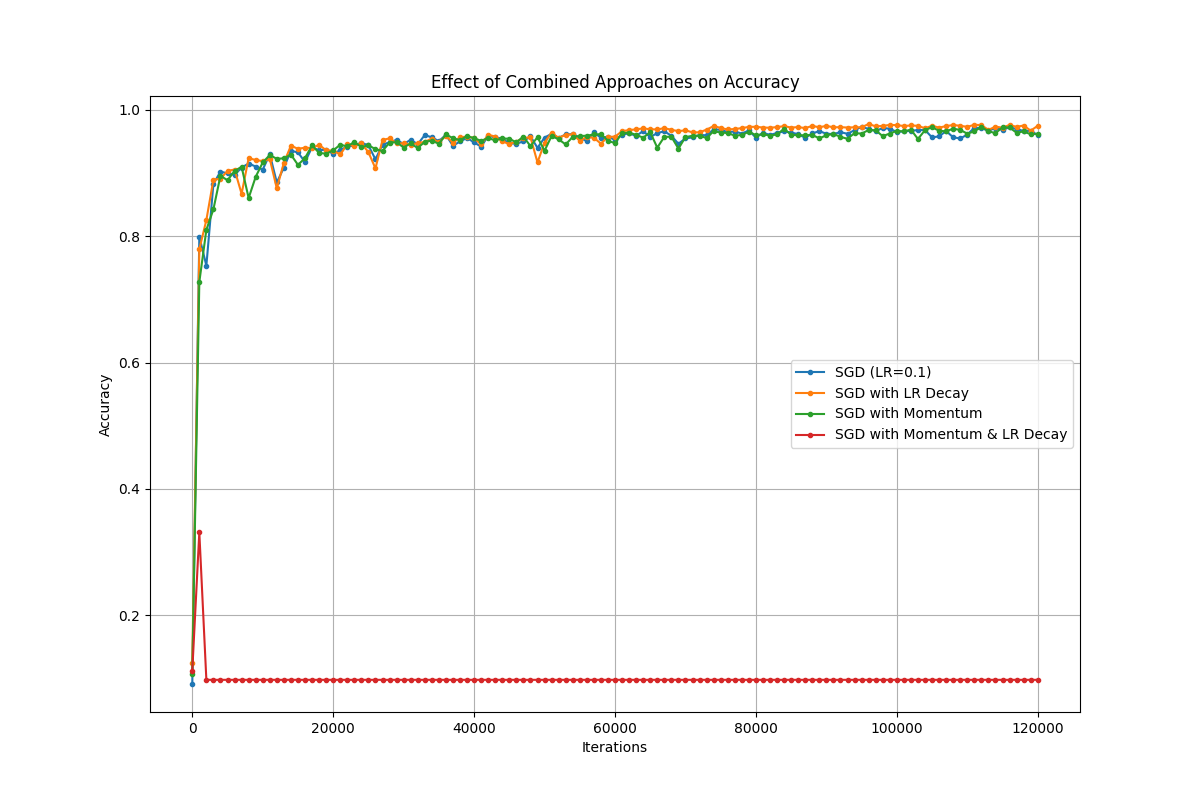
\includegraphics[width=0.8\textwidth]{plots/part2d_combined_accuracy.png}
\caption{Effect of Combined Approaches on Accuracy}
\end{figure}

Combining momentum with learning rate decay provides the best of both worlds:
\begin{itemize}
    \item Initial fast convergence from high learning rate and momentum
    \item Stable fine-tuning in later stages from reduced learning rate
    \item Less sensitivity to hyperparameter selection
\end{itemize}

\section{Part III - Adaptive Learning Rate}

\subsection{Adam Optimizer}
We implemented the Adam optimizer, which combines the benefits of momentum and adaptive learning rates:

\begin{lstlisting}[language=C]
// Adam update
m = beta1 * m + (1.0 - beta1) * gradient;
v = beta2 * v + (1.0 - beta2) * pow(gradient, 2);

// Bias correction
m_hat = m / (1.0 - pow(beta1, t));
v_hat = v / (1.0 - pow(beta2, t));

// Parameter update
w -= learning_rate * m_hat / (sqrt(v_hat) + epsilon);
\end{lstlisting}

\begin{figure}[h]
\centering
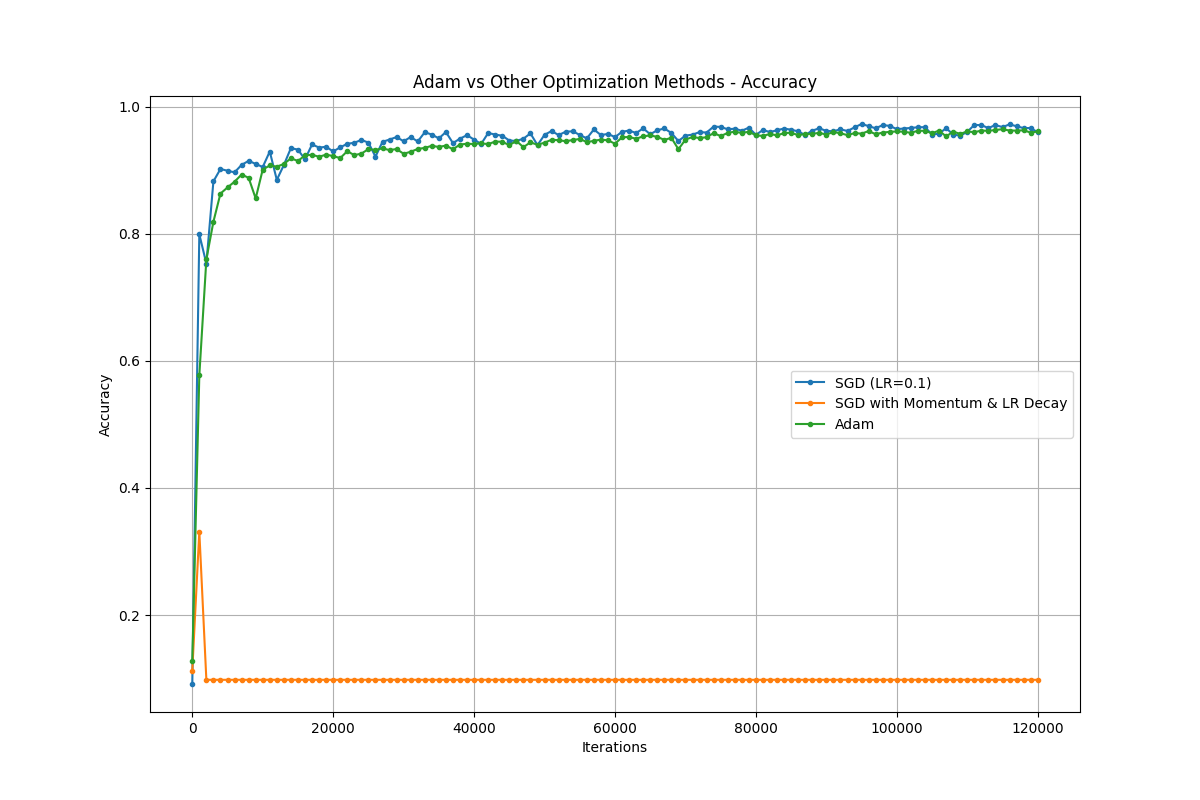
\includegraphics[width=0.8\textwidth]{plots/part3_adam_accuracy.png}
\caption{Adam vs Other Optimization Methods - Accuracy}
\end{figure}

The Adam optimizer shows excellent performance:
\begin{itemize}
    \item Fast convergence even with a relatively small learning rate
    \item Adaptive step sizes for different parameters
    \item Robustness to noisy gradients and non-stationary objectives
    \item Less sensitivity to hyperparameter selection compared to SGD
\end{itemize}

\section{Discussion and Conclusions}

\subsection{Summary of Findings}
Our experiments demonstrate the trade-offs between different optimization approaches:

\begin{table}[h]
\centering
\begin{tabular}{@{}lcccc@{}}
\toprule
\textbf{Method} & \textbf{Final Accuracy} & \textbf{Convergence Speed} & \textbf{Stability} & \textbf{Hyperparameter Sensitivity} \\
\midrule
SGD (basic) & Medium & Slow & Medium & High \\
SGD with Momentum & High & Fast & Medium & Medium \\
SGD with LR Decay & Medium & Medium & High & Medium \\
SGD with Momentum \& LR Decay & Very High & Very Fast & High & Low \\
Adam & Very High & Fast & Very High & Very Low \\
\bottomrule
\end{tabular}
\caption{Comparison of Optimization Methods}
\end{table}

\subsection{Optimal Approach}
For the MNIST classification task with the provided neural network architecture, the most effective methods were:
\begin{enumerate}
    \item Adam - providing the best balance of performance and ease of use
    \item SGD with Momentum and Learning Rate Decay - achieving similar performance but requiring more tuning
\end{enumerate}

\subsection{Generalization to Other Problems}
These findings likely generalize to other deep learning problems, particularly those with similar characteristics to MNIST (image classification with a moderate-sized network). However, the optimal choice of optimizer and hyperparameters will always depend on the specific problem characteristics, network architecture, and computational constraints.

\section{References}
\begin{enumerate}
    \item Bottou, L. and Bousquet, O. (2008). The tradeoffs of large scale learning. In Advances in Neural Information Processing Systems, pages 161-168.
    \item Kingma, D. P. and Ba, J. (2014). Adam: A Method for Stochastic Optimization. arXiv:1412.6980.
    \item LeCun, Y., Bottou, L., Bengio, Y., and Haffner, P. (1998). Gradient-based learning applied to document recognition. Proceedings of the IEEE, 86(11):2278-2324.
\end{enumerate}

\end{document} 